% CNETA at a glance: what the tools do, on one line. The detailed version
% with every file and mode is cneta-pipeline.tex; read this one first.
%
% Plain pdflatex on TeX Live "basic". ./build.sh renders both schemes:
%
%   pdflatex -jobname=cneta-overview-dark \
%     "\def\PipelineScheme{dark}% CNETA at a glance: what the tools do, on one line. The detailed version
% with every file and mode is cneta-pipeline.tex; read this one first.
%
% Plain pdflatex on TeX Live "basic". ./build.sh renders both schemes:
%
%   pdflatex -jobname=cneta-overview-dark \
%     "\def\PipelineScheme{dark}% CNETA at a glance: what the tools do, on one line. The detailed version
% with every file and mode is cneta-pipeline.tex; read this one first.
%
% Plain pdflatex on TeX Live "basic". ./build.sh renders both schemes:
%
%   pdflatex -jobname=cneta-overview-dark \
%     "\def\PipelineScheme{dark}% CNETA at a glance: what the tools do, on one line. The detailed version
% with every file and mode is cneta-pipeline.tex; read this one first.
%
% Plain pdflatex on TeX Live "basic". ./build.sh renders both schemes:
%
%   pdflatex -jobname=cneta-overview-dark \
%     "\def\PipelineScheme{dark}\input{cneta-overview}"
%
%   \PipelineScheme  light | dark   (default light)

\providecommand\PipelineScheme{light}

\documentclass[tikz,border=5mm]{standalone}
\usepackage[T1]{fontenc}
\usepackage{lmodern}
\renewcommand*\familydefault{\sfdefault}
\usetikzlibrary{arrows.meta,positioning,calc,shapes.misc}
\hyphenpenalty=10000
\exhyphenpenalty=10000

% ---------------------------------------------------------------- palette
\def\schemeLight{light}
\ifx\PipelineScheme\schemeLight
  \definecolor{ink}{HTML}{16222E}  \definecolor{muted}{HTML}{6B7280}
  \definecolor{stln}{HTML}{24405C} \definecolor{stfl}{HTML}{E7EEF5}
  \definecolor{syln}{HTML}{55606D} \definecolor{syfl}{HTML}{EDEFF2}
  \definecolor{deln}{HTML}{A5690C} \definecolor{defl}{HTML}{FDF3E2}
  \definecolor{galn}{HTML}{A83226} \definecolor{gafl}{HTML}{FAE9E7}
  \definecolor{opln}{HTML}{2C6B4F} \definecolor{opfl}{HTML}{E6F1EB}
\else
  \definecolor{ink}{HTML}{E6EBF0}  \definecolor{muted}{HTML}{A9B4BF}
  \definecolor{stln}{HTML}{8FB3D9} \definecolor{stfl}{HTML}{25364A}
  \definecolor{syln}{HTML}{A0AAB5} \definecolor{syfl}{HTML}{333B45}
  \definecolor{deln}{HTML}{E0A94B} \definecolor{defl}{HTML}{40321A}
  \definecolor{galn}{HTML}{E07A6E} \definecolor{gafl}{HTML}{42241F}
  \definecolor{opln}{HTML}{6FBF93} \definecolor{opfl}{HTML}{1F3A2B}
\fi

% ---------------------------------------------------------------- styles
\tikzset{
  x=1mm, y=1mm,
  every node/.style={text=ink, font=\normalsize, align=center, inner sep=6pt,
                     rounded corners=3pt, line width=1pt},
  prog/.style={draw=stln, fill=stfl, line width=1.2pt},
  file/.style={draw=syln, fill=syfl},
  result/.style={draw=opln, fill=opfl, line width=1.2pt},
  draft/.style={draw=galn, fill=gafl, dash pattern=on 3pt off 2pt},
  planned/.style={draw=deln, fill=defl, dash pattern=on 3pt off 2pt},
  head/.style={font=\large\bfseries, inner sep=0pt},
  dcap/.style={text=muted, font=\small, inner sep=1pt},
  arr/.style={-{Stealth[length=3mm,width=2.2mm]}, line width=1.2pt, draw=stln},
  arro/.style={-{Stealth[length=3mm,width=2.2mm]}, line width=1.2pt, draw=opln},
  arrd/.style={-{Stealth[length=3mm,width=2.2mm]}, line width=1pt, draw=galn,
               dash pattern=on 3pt off 2pt},
  % legend swatch: a small box in one of the styles above
  chip/.style={minimum width=8mm, minimum height=4.2mm, inner sep=0pt,
               rounded corners=1pt},
  lg/.style={anchor=west, text=ink, font=\small, inner sep=1pt},
}

\begin{document}
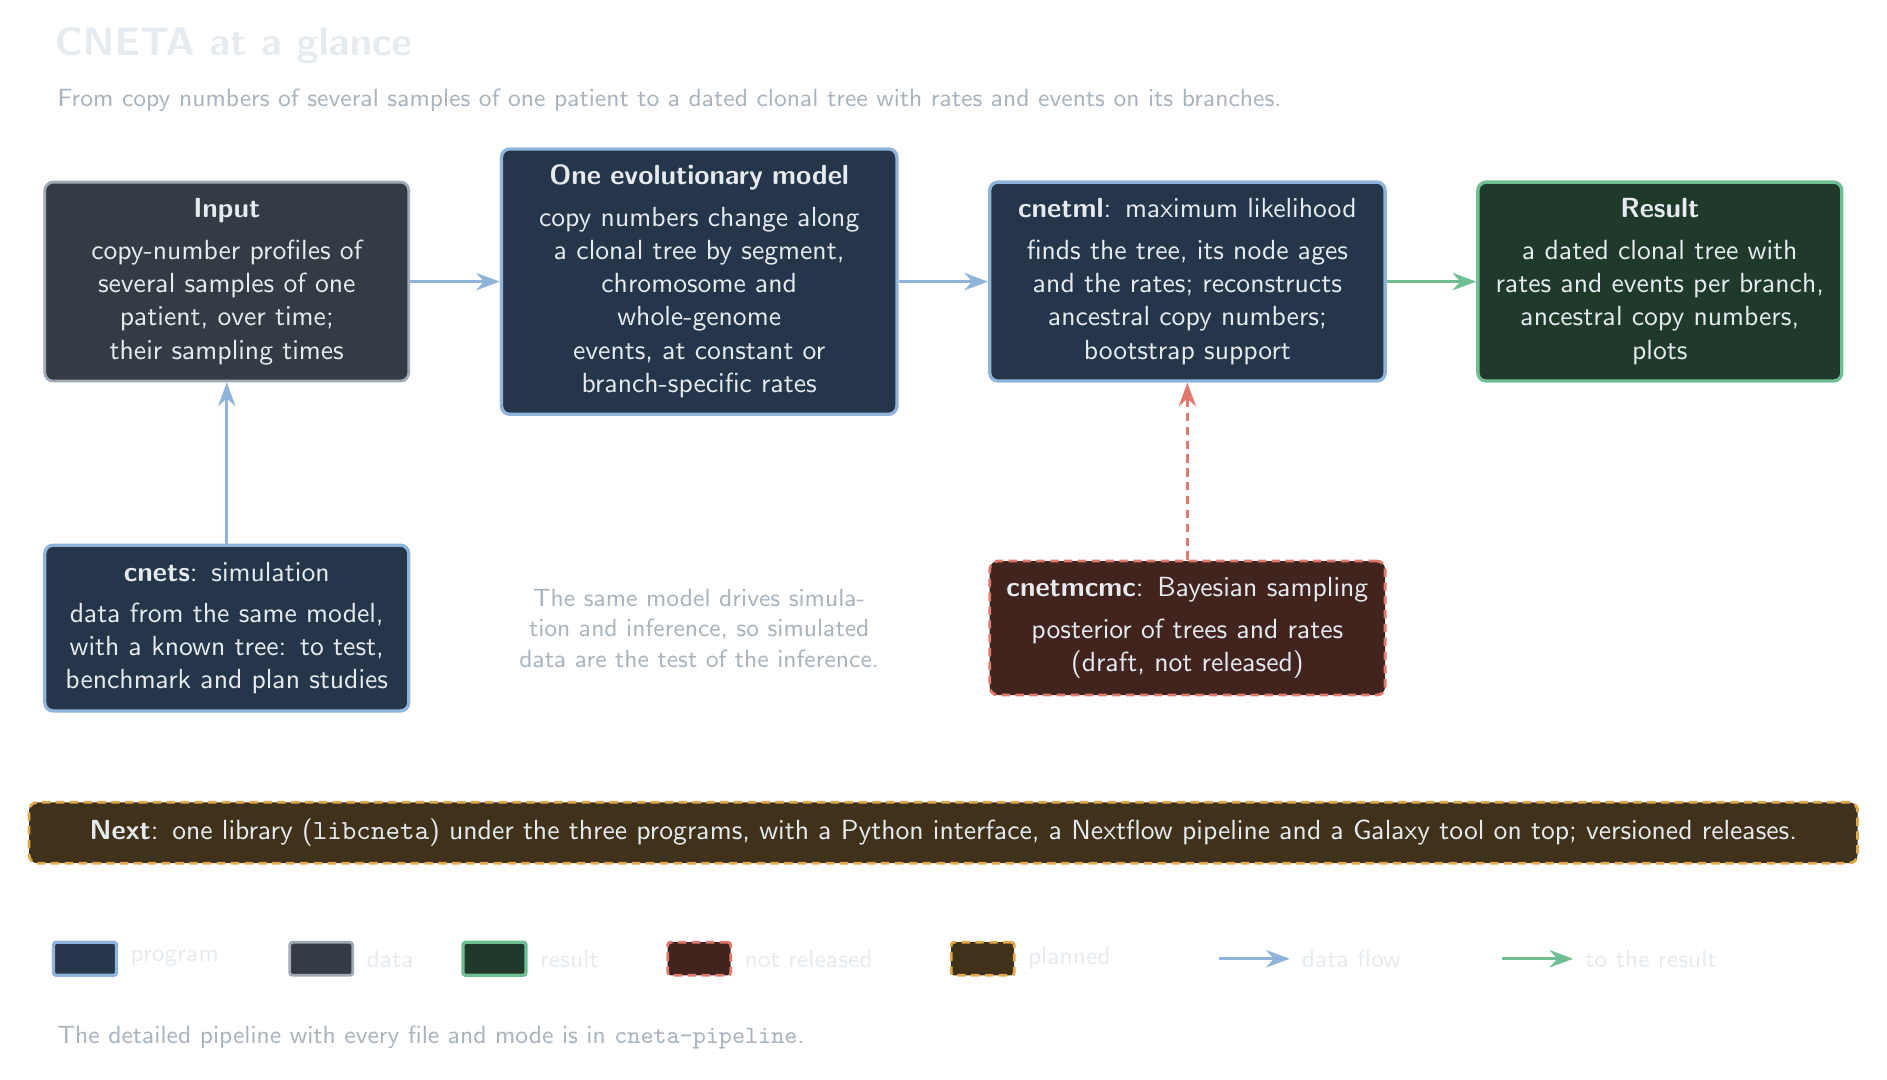
\begin{tikzpicture}

\node[anchor=west, font=\Large\bfseries, inner sep=0pt] at (0,30)
  {CNETA at a glance};
\node[anchor=west, dcap] at (0,23)
  {From copy numbers of several samples of one patient to a dated clonal tree with rates and events on its branches.};

% ---------------------------------------------------------------- main line
\node[file, text width=42mm] (in) at (22,0)
  {\textbf{Input}\\[3pt]copy-number profiles of\\several samples of one\\patient, over time;\\their sampling times};

\node[prog, text width=46mm] (model) at (82,0)
  {\textbf{One evolutionary model}\\[3pt]copy numbers change along\\a clonal tree by segment,\\chromosome and whole-genome\\events, at constant or\\branch-specific rates};

\node[prog, text width=46mm] (ml) at (144,0)
  {\textbf{cnetml}: maximum likelihood\\[3pt]finds the tree, its node ages\\and the rates; reconstructs\\ancestral copy numbers;\\bootstrap support};

\node[result, text width=42mm] (out) at (204,0)
  {\textbf{Result}\\[3pt]a dated clonal tree with\\rates and events per branch,\\ancestral copy numbers,\\plots};

\draw[arr] (in) -- (model);
\draw[arr] (model) -- (ml);
\draw[arro] (ml) -- (out);

% ---------------------------------------------------------------- second line
\node[prog, text width=42mm] (sim) at (22,-44)
  {\textbf{cnets}: simulation\\[3pt]data from the same model,\\with a known tree: to test,\\benchmark and plan studies};
\draw[arr] (sim) -- (in);

\node[draft, text width=46mm] (mcmc) at (144,-44)
  {\textbf{cnetmcmc}: Bayesian sampling\\[3pt]posterior of trees and rates\\(draft, not released)};
\draw[arrd] (mcmc) -- (ml);

\node[dcap, text width=46mm] at (82,-44)
  {The same model drives simulation and inference, so simulated data are the test of the inference.};

% ---------------------------------------------------------------- planned
\node[planned, text width=228mm, font=\normalsize] (next) at (113,-70)
  {\textbf{Next}: one library (\texttt{libcneta}) under the three programs, with a Python interface, a Nextflow pipeline and a Galaxy tool on top; versioned releases.};

% ---------------------------------------------------------------- legend
\begin{scope}[shift={(0,-86)}]
  \node[prog, chip]    (lg1) at (4,0)   {}; \node[lg] at ([xshift=3pt]lg1.east) {program};
  \node[file, chip]    (lg2) at (34,0)  {}; \node[lg] at ([xshift=3pt]lg2.east) {data};
  \node[result, chip]  (lg3) at (56,0)  {}; \node[lg] at ([xshift=3pt]lg3.east) {result};
  \node[draft, chip]   (lg4) at (82,0)  {}; \node[lg] at ([xshift=3pt]lg4.east) {not released};
  \node[planned, chip] (lg5) at (118,0) {}; \node[lg] at ([xshift=3pt]lg5.east) {planned};
  \draw[arr]  (148,0) -- ++(9,0); \node[lg] at (158,0) {data flow};
  \draw[arro] (184,0) -- ++(9,0); \node[lg] at (194,0) {to the result};
\end{scope}
\node[dcap, anchor=west] at (0,-96)
  {The detailed pipeline with every file and mode is in \texttt{cneta-pipeline}.};

\end{tikzpicture}
\end{document}
"
%
%   \PipelineScheme  light | dark   (default light)

\providecommand\PipelineScheme{light}

\documentclass[tikz,border=5mm]{standalone}
\usepackage[T1]{fontenc}
\usepackage{lmodern}
\renewcommand*\familydefault{\sfdefault}
\usetikzlibrary{arrows.meta,positioning,calc,shapes.misc}
\hyphenpenalty=10000
\exhyphenpenalty=10000

% ---------------------------------------------------------------- palette
\def\schemeLight{light}
\ifx\PipelineScheme\schemeLight
  \definecolor{ink}{HTML}{16222E}  \definecolor{muted}{HTML}{6B7280}
  \definecolor{stln}{HTML}{24405C} \definecolor{stfl}{HTML}{E7EEF5}
  \definecolor{syln}{HTML}{55606D} \definecolor{syfl}{HTML}{EDEFF2}
  \definecolor{deln}{HTML}{A5690C} \definecolor{defl}{HTML}{FDF3E2}
  \definecolor{galn}{HTML}{A83226} \definecolor{gafl}{HTML}{FAE9E7}
  \definecolor{opln}{HTML}{2C6B4F} \definecolor{opfl}{HTML}{E6F1EB}
\else
  \definecolor{ink}{HTML}{E6EBF0}  \definecolor{muted}{HTML}{A9B4BF}
  \definecolor{stln}{HTML}{8FB3D9} \definecolor{stfl}{HTML}{25364A}
  \definecolor{syln}{HTML}{A0AAB5} \definecolor{syfl}{HTML}{333B45}
  \definecolor{deln}{HTML}{E0A94B} \definecolor{defl}{HTML}{40321A}
  \definecolor{galn}{HTML}{E07A6E} \definecolor{gafl}{HTML}{42241F}
  \definecolor{opln}{HTML}{6FBF93} \definecolor{opfl}{HTML}{1F3A2B}
\fi

% ---------------------------------------------------------------- styles
\tikzset{
  x=1mm, y=1mm,
  every node/.style={text=ink, font=\normalsize, align=center, inner sep=6pt,
                     rounded corners=3pt, line width=1pt},
  prog/.style={draw=stln, fill=stfl, line width=1.2pt},
  file/.style={draw=syln, fill=syfl},
  result/.style={draw=opln, fill=opfl, line width=1.2pt},
  draft/.style={draw=galn, fill=gafl, dash pattern=on 3pt off 2pt},
  planned/.style={draw=deln, fill=defl, dash pattern=on 3pt off 2pt},
  head/.style={font=\large\bfseries, inner sep=0pt},
  dcap/.style={text=muted, font=\small, inner sep=1pt},
  arr/.style={-{Stealth[length=3mm,width=2.2mm]}, line width=1.2pt, draw=stln},
  arro/.style={-{Stealth[length=3mm,width=2.2mm]}, line width=1.2pt, draw=opln},
  arrd/.style={-{Stealth[length=3mm,width=2.2mm]}, line width=1pt, draw=galn,
               dash pattern=on 3pt off 2pt},
  % legend swatch: a small box in one of the styles above
  chip/.style={minimum width=8mm, minimum height=4.2mm, inner sep=0pt,
               rounded corners=1pt},
  lg/.style={anchor=west, text=ink, font=\small, inner sep=1pt},
}

\begin{document}
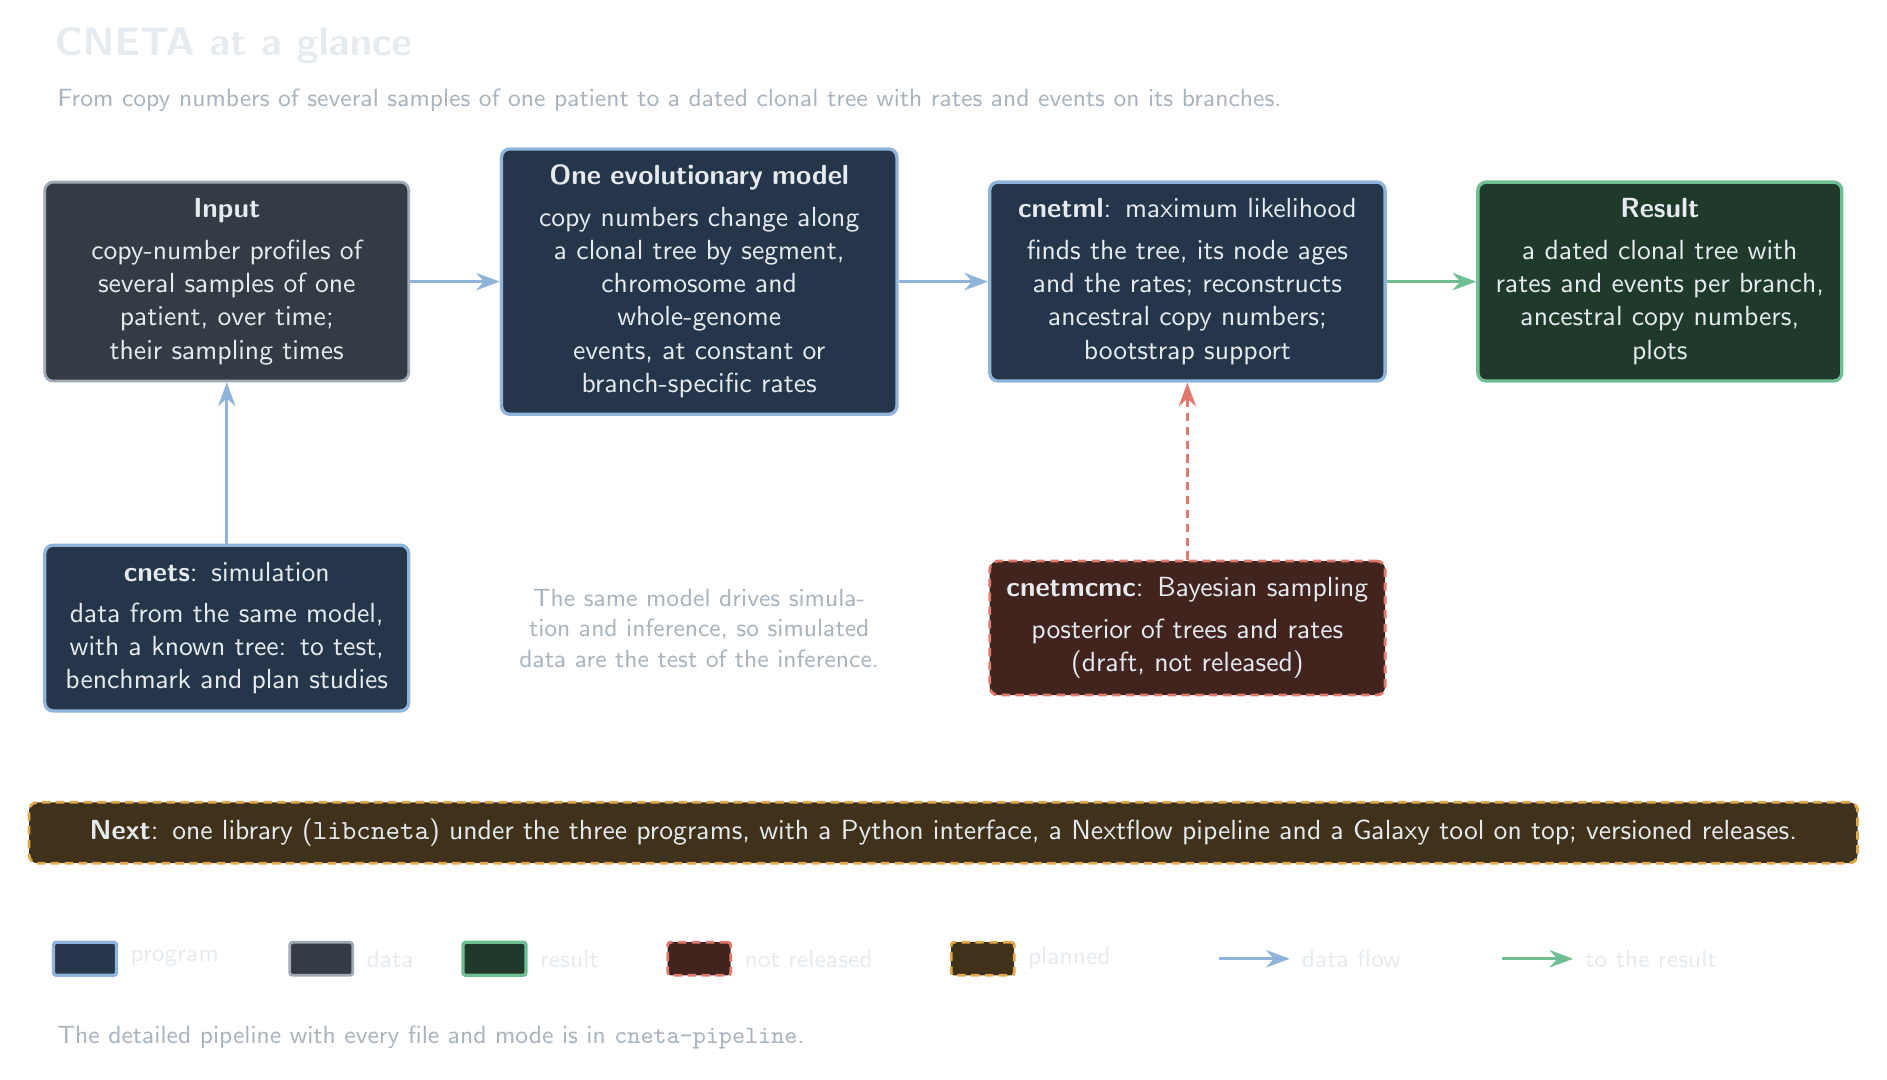
\begin{tikzpicture}

\node[anchor=west, font=\Large\bfseries, inner sep=0pt] at (0,30)
  {CNETA at a glance};
\node[anchor=west, dcap] at (0,23)
  {From copy numbers of several samples of one patient to a dated clonal tree with rates and events on its branches.};

% ---------------------------------------------------------------- main line
\node[file, text width=42mm] (in) at (22,0)
  {\textbf{Input}\\[3pt]copy-number profiles of\\several samples of one\\patient, over time;\\their sampling times};

\node[prog, text width=46mm] (model) at (82,0)
  {\textbf{One evolutionary model}\\[3pt]copy numbers change along\\a clonal tree by segment,\\chromosome and whole-genome\\events, at constant or\\branch-specific rates};

\node[prog, text width=46mm] (ml) at (144,0)
  {\textbf{cnetml}: maximum likelihood\\[3pt]finds the tree, its node ages\\and the rates; reconstructs\\ancestral copy numbers;\\bootstrap support};

\node[result, text width=42mm] (out) at (204,0)
  {\textbf{Result}\\[3pt]a dated clonal tree with\\rates and events per branch,\\ancestral copy numbers,\\plots};

\draw[arr] (in) -- (model);
\draw[arr] (model) -- (ml);
\draw[arro] (ml) -- (out);

% ---------------------------------------------------------------- second line
\node[prog, text width=42mm] (sim) at (22,-44)
  {\textbf{cnets}: simulation\\[3pt]data from the same model,\\with a known tree: to test,\\benchmark and plan studies};
\draw[arr] (sim) -- (in);

\node[draft, text width=46mm] (mcmc) at (144,-44)
  {\textbf{cnetmcmc}: Bayesian sampling\\[3pt]posterior of trees and rates\\(draft, not released)};
\draw[arrd] (mcmc) -- (ml);

\node[dcap, text width=46mm] at (82,-44)
  {The same model drives simulation and inference, so simulated data are the test of the inference.};

% ---------------------------------------------------------------- planned
\node[planned, text width=228mm, font=\normalsize] (next) at (113,-70)
  {\textbf{Next}: one library (\texttt{libcneta}) under the three programs, with a Python interface, a Nextflow pipeline and a Galaxy tool on top; versioned releases.};

% ---------------------------------------------------------------- legend
\begin{scope}[shift={(0,-86)}]
  \node[prog, chip]    (lg1) at (4,0)   {}; \node[lg] at ([xshift=3pt]lg1.east) {program};
  \node[file, chip]    (lg2) at (34,0)  {}; \node[lg] at ([xshift=3pt]lg2.east) {data};
  \node[result, chip]  (lg3) at (56,0)  {}; \node[lg] at ([xshift=3pt]lg3.east) {result};
  \node[draft, chip]   (lg4) at (82,0)  {}; \node[lg] at ([xshift=3pt]lg4.east) {not released};
  \node[planned, chip] (lg5) at (118,0) {}; \node[lg] at ([xshift=3pt]lg5.east) {planned};
  \draw[arr]  (148,0) -- ++(9,0); \node[lg] at (158,0) {data flow};
  \draw[arro] (184,0) -- ++(9,0); \node[lg] at (194,0) {to the result};
\end{scope}
\node[dcap, anchor=west] at (0,-96)
  {The detailed pipeline with every file and mode is in \texttt{cneta-pipeline}.};

\end{tikzpicture}
\end{document}
"
%
%   \PipelineScheme  light | dark   (default light)

\providecommand\PipelineScheme{light}

\documentclass[tikz,border=5mm]{standalone}
\usepackage[T1]{fontenc}
\usepackage{lmodern}
\renewcommand*\familydefault{\sfdefault}
\usetikzlibrary{arrows.meta,positioning,calc,shapes.misc}
\hyphenpenalty=10000
\exhyphenpenalty=10000

% ---------------------------------------------------------------- palette
\def\schemeLight{light}
\ifx\PipelineScheme\schemeLight
  \definecolor{ink}{HTML}{16222E}  \definecolor{muted}{HTML}{6B7280}
  \definecolor{stln}{HTML}{24405C} \definecolor{stfl}{HTML}{E7EEF5}
  \definecolor{syln}{HTML}{55606D} \definecolor{syfl}{HTML}{EDEFF2}
  \definecolor{deln}{HTML}{A5690C} \definecolor{defl}{HTML}{FDF3E2}
  \definecolor{galn}{HTML}{A83226} \definecolor{gafl}{HTML}{FAE9E7}
  \definecolor{opln}{HTML}{2C6B4F} \definecolor{opfl}{HTML}{E6F1EB}
\else
  \definecolor{ink}{HTML}{E6EBF0}  \definecolor{muted}{HTML}{A9B4BF}
  \definecolor{stln}{HTML}{8FB3D9} \definecolor{stfl}{HTML}{25364A}
  \definecolor{syln}{HTML}{A0AAB5} \definecolor{syfl}{HTML}{333B45}
  \definecolor{deln}{HTML}{E0A94B} \definecolor{defl}{HTML}{40321A}
  \definecolor{galn}{HTML}{E07A6E} \definecolor{gafl}{HTML}{42241F}
  \definecolor{opln}{HTML}{6FBF93} \definecolor{opfl}{HTML}{1F3A2B}
\fi

% ---------------------------------------------------------------- styles
\tikzset{
  x=1mm, y=1mm,
  every node/.style={text=ink, font=\normalsize, align=center, inner sep=6pt,
                     rounded corners=3pt, line width=1pt},
  prog/.style={draw=stln, fill=stfl, line width=1.2pt},
  file/.style={draw=syln, fill=syfl},
  result/.style={draw=opln, fill=opfl, line width=1.2pt},
  draft/.style={draw=galn, fill=gafl, dash pattern=on 3pt off 2pt},
  planned/.style={draw=deln, fill=defl, dash pattern=on 3pt off 2pt},
  head/.style={font=\large\bfseries, inner sep=0pt},
  dcap/.style={text=muted, font=\small, inner sep=1pt},
  arr/.style={-{Stealth[length=3mm,width=2.2mm]}, line width=1.2pt, draw=stln},
  arro/.style={-{Stealth[length=3mm,width=2.2mm]}, line width=1.2pt, draw=opln},
  arrd/.style={-{Stealth[length=3mm,width=2.2mm]}, line width=1pt, draw=galn,
               dash pattern=on 3pt off 2pt},
  % legend swatch: a small box in one of the styles above
  chip/.style={minimum width=8mm, minimum height=4.2mm, inner sep=0pt,
               rounded corners=1pt},
  lg/.style={anchor=west, text=ink, font=\small, inner sep=1pt},
}

\begin{document}
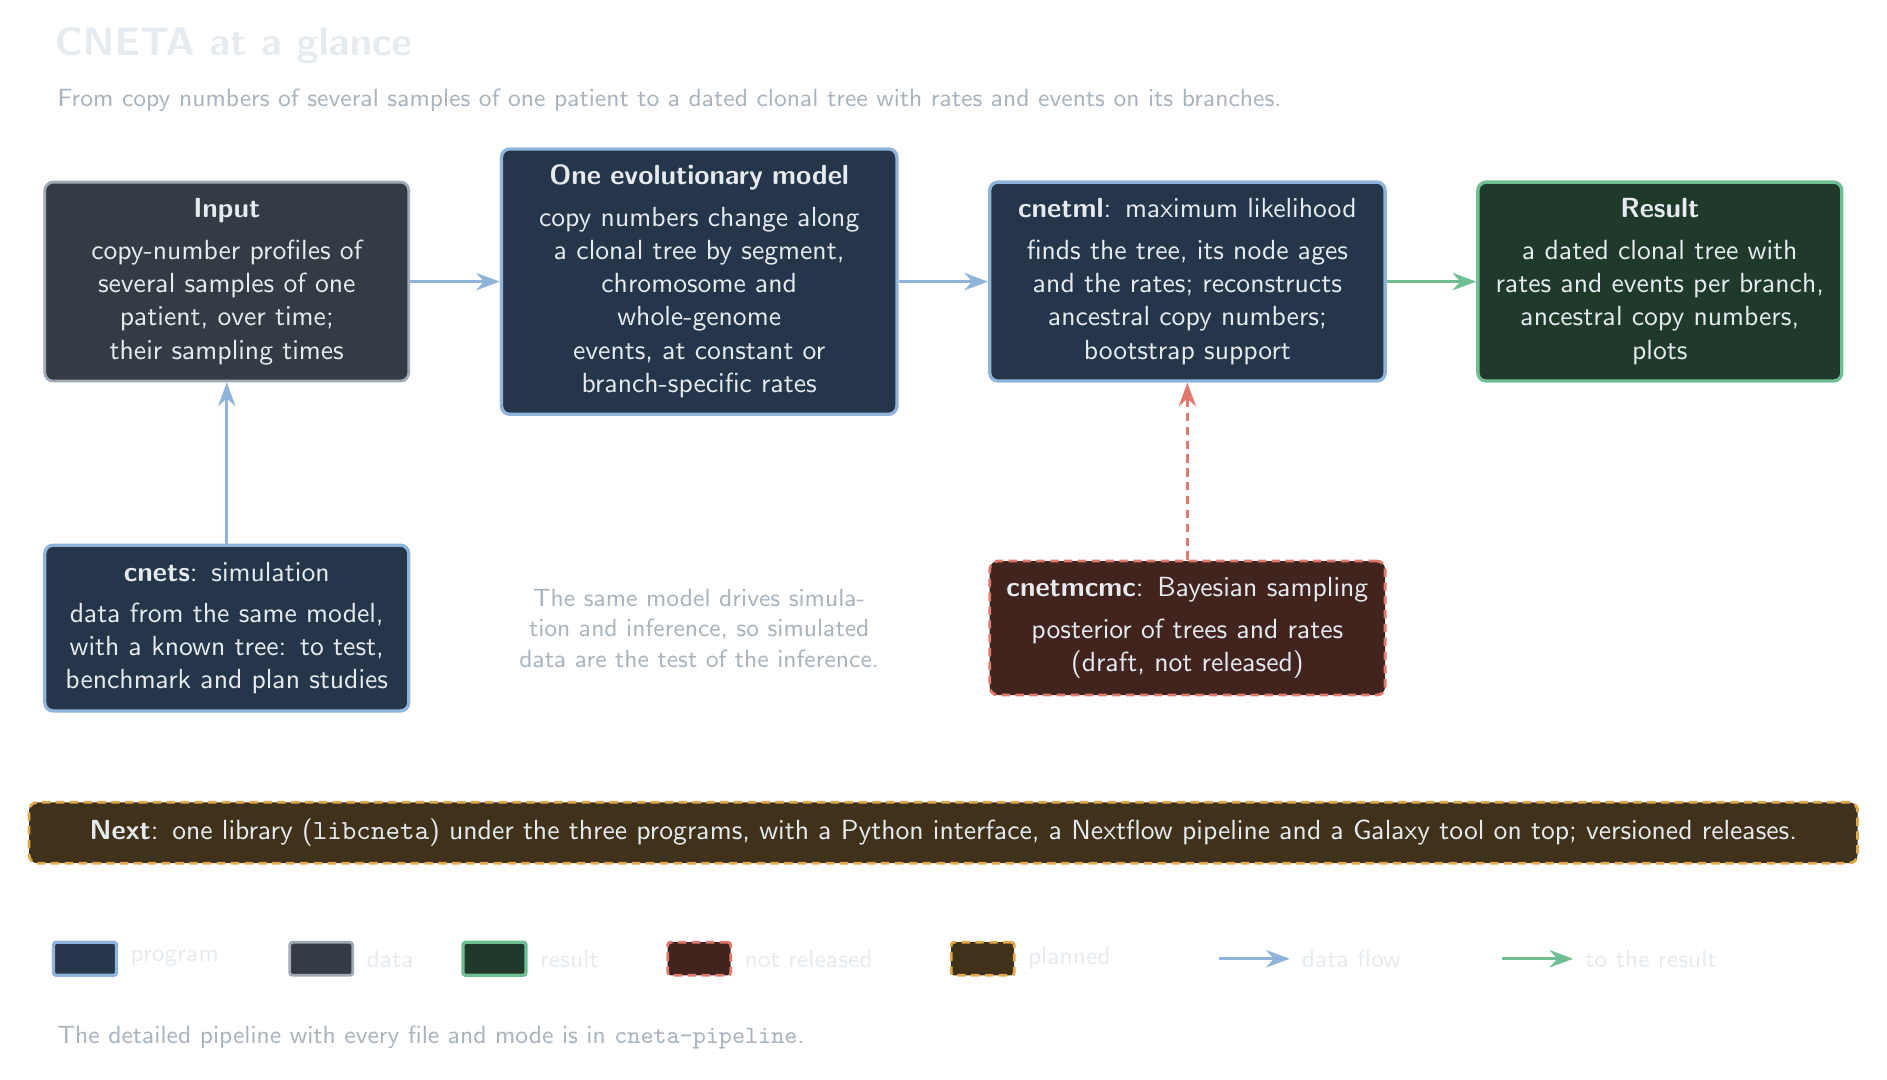
\begin{tikzpicture}

\node[anchor=west, font=\Large\bfseries, inner sep=0pt] at (0,30)
  {CNETA at a glance};
\node[anchor=west, dcap] at (0,23)
  {From copy numbers of several samples of one patient to a dated clonal tree with rates and events on its branches.};

% ---------------------------------------------------------------- main line
\node[file, text width=42mm] (in) at (22,0)
  {\textbf{Input}\\[3pt]copy-number profiles of\\several samples of one\\patient, over time;\\their sampling times};

\node[prog, text width=46mm] (model) at (82,0)
  {\textbf{One evolutionary model}\\[3pt]copy numbers change along\\a clonal tree by segment,\\chromosome and whole-genome\\events, at constant or\\branch-specific rates};

\node[prog, text width=46mm] (ml) at (144,0)
  {\textbf{cnetml}: maximum likelihood\\[3pt]finds the tree, its node ages\\and the rates; reconstructs\\ancestral copy numbers;\\bootstrap support};

\node[result, text width=42mm] (out) at (204,0)
  {\textbf{Result}\\[3pt]a dated clonal tree with\\rates and events per branch,\\ancestral copy numbers,\\plots};

\draw[arr] (in) -- (model);
\draw[arr] (model) -- (ml);
\draw[arro] (ml) -- (out);

% ---------------------------------------------------------------- second line
\node[prog, text width=42mm] (sim) at (22,-44)
  {\textbf{cnets}: simulation\\[3pt]data from the same model,\\with a known tree: to test,\\benchmark and plan studies};
\draw[arr] (sim) -- (in);

\node[draft, text width=46mm] (mcmc) at (144,-44)
  {\textbf{cnetmcmc}: Bayesian sampling\\[3pt]posterior of trees and rates\\(draft, not released)};
\draw[arrd] (mcmc) -- (ml);

\node[dcap, text width=46mm] at (82,-44)
  {The same model drives simulation and inference, so simulated data are the test of the inference.};

% ---------------------------------------------------------------- planned
\node[planned, text width=228mm, font=\normalsize] (next) at (113,-70)
  {\textbf{Next}: one library (\texttt{libcneta}) under the three programs, with a Python interface, a Nextflow pipeline and a Galaxy tool on top; versioned releases.};

% ---------------------------------------------------------------- legend
\begin{scope}[shift={(0,-86)}]
  \node[prog, chip]    (lg1) at (4,0)   {}; \node[lg] at ([xshift=3pt]lg1.east) {program};
  \node[file, chip]    (lg2) at (34,0)  {}; \node[lg] at ([xshift=3pt]lg2.east) {data};
  \node[result, chip]  (lg3) at (56,0)  {}; \node[lg] at ([xshift=3pt]lg3.east) {result};
  \node[draft, chip]   (lg4) at (82,0)  {}; \node[lg] at ([xshift=3pt]lg4.east) {not released};
  \node[planned, chip] (lg5) at (118,0) {}; \node[lg] at ([xshift=3pt]lg5.east) {planned};
  \draw[arr]  (148,0) -- ++(9,0); \node[lg] at (158,0) {data flow};
  \draw[arro] (184,0) -- ++(9,0); \node[lg] at (194,0) {to the result};
\end{scope}
\node[dcap, anchor=west] at (0,-96)
  {The detailed pipeline with every file and mode is in \texttt{cneta-pipeline}.};

\end{tikzpicture}
\end{document}
"
%
%   \PipelineScheme  light | dark   (default light)

\providecommand\PipelineScheme{light}

\documentclass[tikz,border=5mm]{standalone}
\usepackage[T1]{fontenc}
\usepackage{lmodern}
\renewcommand*\familydefault{\sfdefault}
\usetikzlibrary{arrows.meta,positioning,calc,shapes.misc}
\hyphenpenalty=10000
\exhyphenpenalty=10000

% ---------------------------------------------------------------- palette
\def\schemeLight{light}
\ifx\PipelineScheme\schemeLight
  \definecolor{ink}{HTML}{16222E}  \definecolor{muted}{HTML}{6B7280}
  \definecolor{stln}{HTML}{24405C} \definecolor{stfl}{HTML}{E7EEF5}
  \definecolor{syln}{HTML}{55606D} \definecolor{syfl}{HTML}{EDEFF2}
  \definecolor{deln}{HTML}{A5690C} \definecolor{defl}{HTML}{FDF3E2}
  \definecolor{galn}{HTML}{A83226} \definecolor{gafl}{HTML}{FAE9E7}
  \definecolor{opln}{HTML}{2C6B4F} \definecolor{opfl}{HTML}{E6F1EB}
\else
  \definecolor{ink}{HTML}{E6EBF0}  \definecolor{muted}{HTML}{A9B4BF}
  \definecolor{stln}{HTML}{8FB3D9} \definecolor{stfl}{HTML}{25364A}
  \definecolor{syln}{HTML}{A0AAB5} \definecolor{syfl}{HTML}{333B45}
  \definecolor{deln}{HTML}{E0A94B} \definecolor{defl}{HTML}{40321A}
  \definecolor{galn}{HTML}{E07A6E} \definecolor{gafl}{HTML}{42241F}
  \definecolor{opln}{HTML}{6FBF93} \definecolor{opfl}{HTML}{1F3A2B}
\fi

% ---------------------------------------------------------------- styles
\tikzset{
  x=1mm, y=1mm,
  every node/.style={text=ink, font=\normalsize, align=center, inner sep=6pt,
                     rounded corners=3pt, line width=1pt},
  prog/.style={draw=stln, fill=stfl, line width=1.2pt},
  file/.style={draw=syln, fill=syfl},
  result/.style={draw=opln, fill=opfl, line width=1.2pt},
  draft/.style={draw=galn, fill=gafl, dash pattern=on 3pt off 2pt},
  planned/.style={draw=deln, fill=defl, dash pattern=on 3pt off 2pt},
  head/.style={font=\large\bfseries, inner sep=0pt},
  dcap/.style={text=muted, font=\small, inner sep=1pt},
  arr/.style={-{Stealth[length=3mm,width=2.2mm]}, line width=1.2pt, draw=stln},
  arro/.style={-{Stealth[length=3mm,width=2.2mm]}, line width=1.2pt, draw=opln},
  arrd/.style={-{Stealth[length=3mm,width=2.2mm]}, line width=1pt, draw=galn,
               dash pattern=on 3pt off 2pt},
  % legend swatch: a small box in one of the styles above
  chip/.style={minimum width=8mm, minimum height=4.2mm, inner sep=0pt,
               rounded corners=1pt},
  lg/.style={anchor=west, text=ink, font=\small, inner sep=1pt},
}

\begin{document}
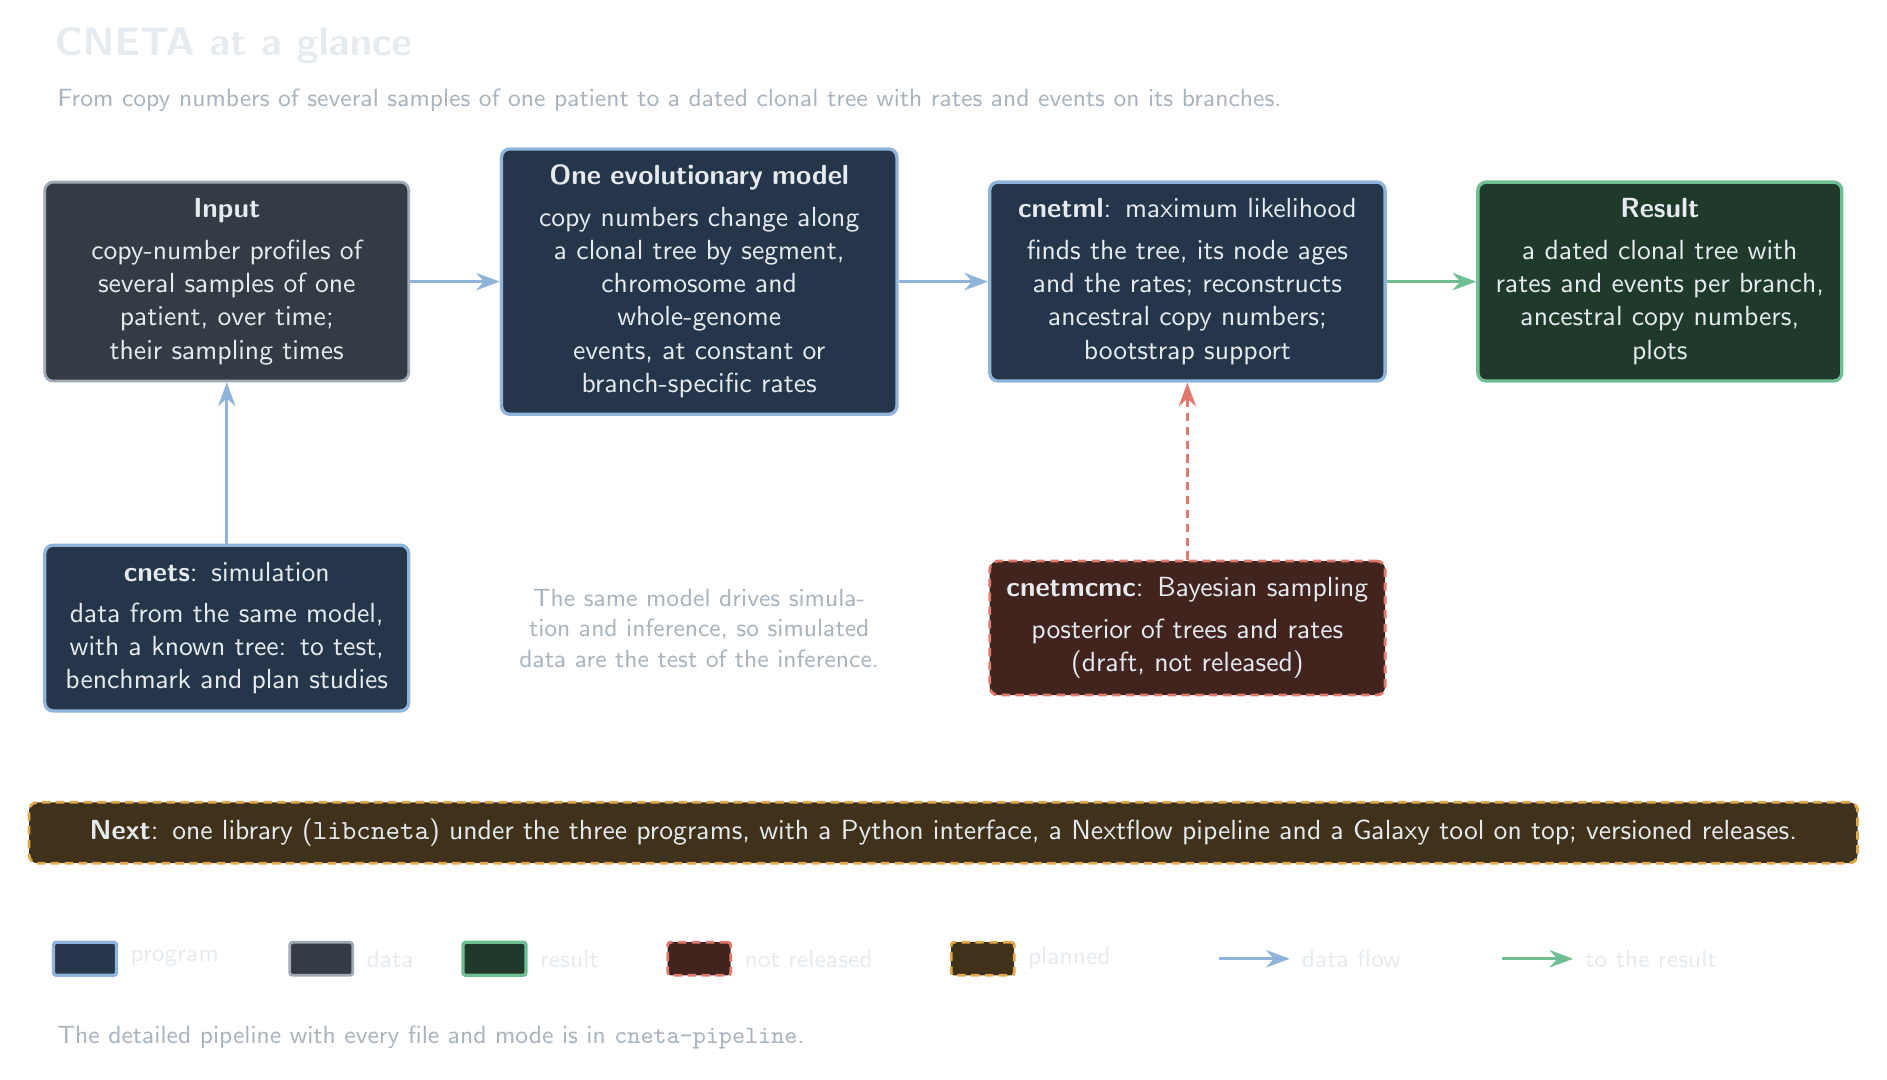
\begin{tikzpicture}

\node[anchor=west, font=\Large\bfseries, inner sep=0pt] at (0,30)
  {CNETA at a glance};
\node[anchor=west, dcap] at (0,23)
  {From copy numbers of several samples of one patient to a dated clonal tree with rates and events on its branches.};

% ---------------------------------------------------------------- main line
\node[file, text width=42mm] (in) at (22,0)
  {\textbf{Input}\\[3pt]copy-number profiles of\\several samples of one\\patient, over time;\\their sampling times};

\node[prog, text width=46mm] (model) at (82,0)
  {\textbf{One evolutionary model}\\[3pt]copy numbers change along\\a clonal tree by segment,\\chromosome and whole-genome\\events, at constant or\\branch-specific rates};

\node[prog, text width=46mm] (ml) at (144,0)
  {\textbf{cnetml}: maximum likelihood\\[3pt]finds the tree, its node ages\\and the rates; reconstructs\\ancestral copy numbers;\\bootstrap support};

\node[result, text width=42mm] (out) at (204,0)
  {\textbf{Result}\\[3pt]a dated clonal tree with\\rates and events per branch,\\ancestral copy numbers,\\plots};

\draw[arr] (in) -- (model);
\draw[arr] (model) -- (ml);
\draw[arro] (ml) -- (out);

% ---------------------------------------------------------------- second line
\node[prog, text width=42mm] (sim) at (22,-44)
  {\textbf{cnets}: simulation\\[3pt]data from the same model,\\with a known tree: to test,\\benchmark and plan studies};
\draw[arr] (sim) -- (in);

\node[draft, text width=46mm] (mcmc) at (144,-44)
  {\textbf{cnetmcmc}: Bayesian sampling\\[3pt]posterior of trees and rates\\(draft, not released)};
\draw[arrd] (mcmc) -- (ml);

\node[dcap, text width=46mm] at (82,-44)
  {The same model drives simulation and inference, so simulated data are the test of the inference.};

% ---------------------------------------------------------------- planned
\node[planned, text width=228mm, font=\normalsize] (next) at (113,-70)
  {\textbf{Next}: one library (\texttt{libcneta}) under the three programs, with a Python interface, a Nextflow pipeline and a Galaxy tool on top; versioned releases.};

% ---------------------------------------------------------------- legend
\begin{scope}[shift={(0,-86)}]
  \node[prog, chip]    (lg1) at (4,0)   {}; \node[lg] at ([xshift=3pt]lg1.east) {program};
  \node[file, chip]    (lg2) at (34,0)  {}; \node[lg] at ([xshift=3pt]lg2.east) {data};
  \node[result, chip]  (lg3) at (56,0)  {}; \node[lg] at ([xshift=3pt]lg3.east) {result};
  \node[draft, chip]   (lg4) at (82,0)  {}; \node[lg] at ([xshift=3pt]lg4.east) {not released};
  \node[planned, chip] (lg5) at (118,0) {}; \node[lg] at ([xshift=3pt]lg5.east) {planned};
  \draw[arr]  (148,0) -- ++(9,0); \node[lg] at (158,0) {data flow};
  \draw[arro] (184,0) -- ++(9,0); \node[lg] at (194,0) {to the result};
\end{scope}
\node[dcap, anchor=west] at (0,-96)
  {The detailed pipeline with every file and mode is in \texttt{cneta-pipeline}.};

\end{tikzpicture}
\end{document}
